\documentclass{standalone}
\usepackage{forsyde-pc}
\usetikzlibrary{decorations.markings}

\begin{document}
\newsavebox{\insignal}
\savebox{\insignal}{
  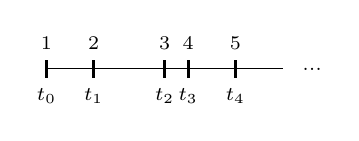
\begin{tikzpicture}[
    sync/.style={fill,inner xsep=0pt},
    decoration={
      markings,
      mark=at position .0 with {\node[sync,label=below:{\scriptsize $t_0$}] {};},
      mark=at position .2 with {\node[sync,label=below:{\scriptsize $t_1$}] {};},
      mark=at position .5 with {\node[sync,label=below:{\scriptsize $t_2$}] {};},
      mark=at position .6 with {\node[sync,label=below:{\scriptsize $t_3$}] {};},
      mark=at position .8 with {\node[sync,label=below:{\scriptsize $t_4$}] {};},
      mark=at position .0 with {\node[label=above:{\scriptsize $1$}] {};},
      mark=at position .2 with {\node[label=above:{\scriptsize $2$}] {};},
      mark=at position .5 with {\node[label=above:{\scriptsize $3$}] {};},
      mark=at position .6 with {\node[label=above:{\scriptsize $4$}] {};},
      mark=at position .8 with {\node[label=above:{\scriptsize $5$}] {};},
      mark=at position 1 with {\node[label=right:{\scriptsize $...$}] {};},
    }
    ]
    \draw[postaction=decorate, ] (0,0) -- (3,0); 
  \end{tikzpicture}
}
\newsavebox{\outsignal}
\savebox{\outsignal}{
  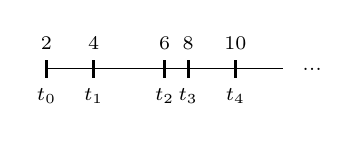
\begin{tikzpicture}[
    sync/.style={fill,inner xsep=0pt},
    decoration={
      markings,
      mark=at position .0 with {\node[sync,label=below:{\scriptsize $t_0$}] {};},
      mark=at position .2 with {\node[sync,label=below:{\scriptsize $t_1$}] {};},
      mark=at position .5 with {\node[sync,label=below:{\scriptsize $t_2$}] {};},
      mark=at position .6 with {\node[sync,label=below:{\scriptsize $t_3$}] {};},
      mark=at position .8 with {\node[sync,label=below:{\scriptsize $t_4$}] {};},
      mark=at position .0 with {\node[label=above:{\scriptsize $2$}] {};},
      mark=at position .2 with {\node[label=above:{\scriptsize $4$}] {};},
      mark=at position .5 with {\node[label=above:{\scriptsize $6$}] {};},
      mark=at position .6 with {\node[label=above:{\scriptsize $8$}] {};},
      mark=at position .8 with {\node[label=above:{\scriptsize $10$}] {};},
      mark=at position 1 with {\node[label=right:{\scriptsize $...$}] {};},
    }
    ]
    \draw[postaction=decorate, ] (0,0) -- (3,0); 
  \end{tikzpicture}
}

\begin{tikzpicture}
  \leafstd[moc=sy, ni=2, no=1, nf=1, f1=$(+)$, type=
comb]{p1}{0,0}{P};
  \node (t1) at ($(p1-p.i1)-(3,-.5)$) {\usebox{\insignal}};
  \node (t2) at ($(p1-p.i2)-(3,.5)$) {\usebox{\insignal}}; 
  \node (t3) at ($(p1-p.o1)+(3,0)$) {\usebox{\outsignal}}; 
 
  \signal[-|-] (t1.east) -> (p1-p.i1); 
  \signal[-|-] (t2.east) -> (p1-p.i2);
  \signal[   ] (p1-p.o1) -> (t3.west);
\end{tikzpicture}  
\end{document}

%%% Local Variables:
%%% mode: latex
%%% TeX-master: t
%%% End:
